% Source: Code/ML_overlay/ir_rgb_registration/paper/ml_overlay_report_materials/ir_rgb_registration_report/figures/fig_optical_flow_constraint.tex
\documentclass[tikz,border=10pt]{standalone}
\usepackage{tikz}
\usetikzlibrary{arrows.meta,positioning,calc}

\definecolor{garnet}{RGB}{115,0,10}
\definecolor{rose}{RGB}{204,46,64}
\definecolor{atlantic}{RGB}{70,106,159}
\definecolor{congaree}{RGB}{31,65,77}
\definecolor{black90}{RGB}{54,54,54}
\definecolor{black70}{RGB}{92,92,92}
\definecolor{black50}{RGB}{162,162,162}

\begin{document}
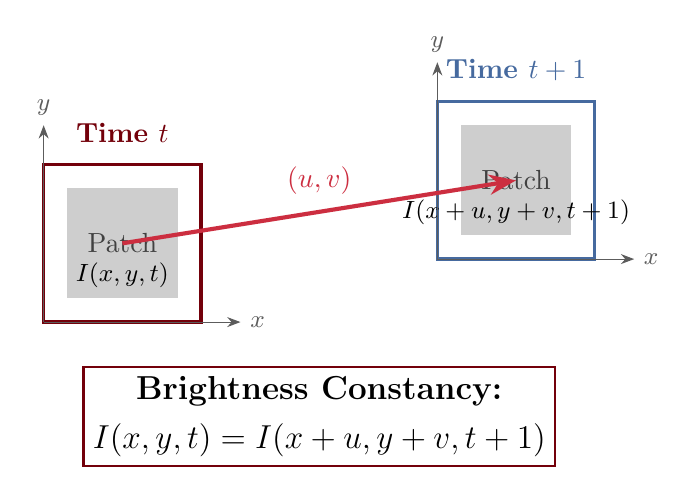
\begin{tikzpicture}[>=Stealth]

    % Time t image patch
    \draw[very thick, garnet] (0,0) rectangle (2,2);
    \node[garnet, font=\bfseries] at (1,2.4) {Time $t$};
    \node[black90] at (1,1) {Patch};
    \fill[black70, opacity=0.3] (0.3,0.3) rectangle (1.7,1.7);
    \node[font=\small] at (1,0.6) {$I(x,y,t)$};

    % Coordinate axes at time t
    \draw[->, black70] (0,0) -- (2.5,0) node[right, font=\small] {$x$};
    \draw[->, black70] (0,0) -- (0,2.5) node[above, font=\small] {$y$};

    % Time t+1 image patch (displaced)
    \draw[very thick, atlantic] (5,0.8) rectangle (7,2.8);
    \node[atlantic, font=\bfseries] at (6,3.2) {Time $t+1$};
    \node[black90] at (6,1.8) {Patch};
    \fill[black70, opacity=0.3] (5.3,1.1) rectangle (6.7,2.5);
    \node[font=\small] at (6,1.4) {$I(x+u, y+v, t+1)$};

    % Coordinate axes at time t+1
    \draw[->, black70] (5,0.8) -- (7.5,0.8) node[right, font=\small] {$x$};
    \draw[->, black70] (5,0.8) -- (5,3.3) node[above, font=\small] {$y$};

    % Displacement vector
    \draw[->, very thick, rose, line width=1.5pt] (1,1) -- (6,1.8);
    \node[rose, font=\bfseries] at (3.5,1.8) {$(u, v)$};

    % Brightness constancy equation
    \node[draw=garnet, thick, fill=white, align=center, font=\large] at (3.5,-1.2) {
        \textbf{Brightness Constancy:} \\[4pt]
        $I(x,y,t) = I(x+u, y+v, t+1)$
    };

\end{tikzpicture}
\end{document}
